% This example poster is from Scientific Career Resources
%
% Author:
% Chris Rackauckas <contact@chrisrackauckas.com>
% http://www.chrisrackauckas.com

\documentclass[papersize={48in,36in},dvipsnames,fontmag=.60]{umbcposter}

\usepackage{multicol}
\usepackage{tikz}
\usepackage{pgfplots}

\usepackage{times}
\usepackage{url}
\usepackage{amsmath}
\definecolor{mitred}{RGB}{163,31,52}
\definecolor{mitdgray}{RGB}{138,139,140}
\definecolor{mitlgray}{RGB}{194,192,191}

% Change the font to Computer Modern Sans Serif
% The default is Times New Roman
\renewcommand{\rmdefault}{cmss}

\begin{document}

\newcommand{\mytitle}{
    \tikz \node[
            fill=white,
            draw=mitred,                   % draw box border
            rounded corners=2ex,
            opacity=0.75,                % background opacity
            text opacity=.9,             % text opacity
            inner sep=0.15\headheight,  % padding around the text
        ] at (0,0) {
            \begin{tabular}{c}
                \Huge Efficient Stiff Ordinary Differential Equation Solvers for \\
                \Huge Quantitative Systems Pharmacology (QsP) \\
                \huge Yingbo Ma, Xingjian Guo, Chris Rackauckas
            \end{tabular}
    };    % don't forget the semicolon here!
}

\posterinit{
	%grid,
	columns = {3},
	background style = {fill = mitlgray},
	title = {\mytitle},
	left logo = {
\includegraphics[height=0.75\headheight]{figures/pumas.pdf}},
	right logo = {
\includegraphics[height=0.5\headheight]{figures/MIT-logo-with-spelling-print-black-red-design1}},
	box/border style= {draw = black, line width = 1pt},
	box/header style = {top color = mitred, bottom color = mitred, middle color = mitred, fill opacity = .9},
	box/header font color = {white},
	box/header font = {\large\rm},
	box/body style = {fill = white, fill opacity=.85},
	head height = {0.15\textheight},
	box/all rounded
}

\boxit{col = 0, at top, name=problem}{Introduction to Stiff ODE}{
  In general, an ordinary differential equation (ODE) can be written in the form
  of
  \[
    u' = f(u, t).
  \]
  In practice, stiff ODEs can be thought as a type of ODEs which explicit
  solvers do not work. Here is an example: the solutions of the equation
  \[
    u' = -50(u - \cos t), \quad u(0) = 0
  \]
  has a rapid transient phase at the beginning.

  \vspace{5pt}
  \begin{center}
    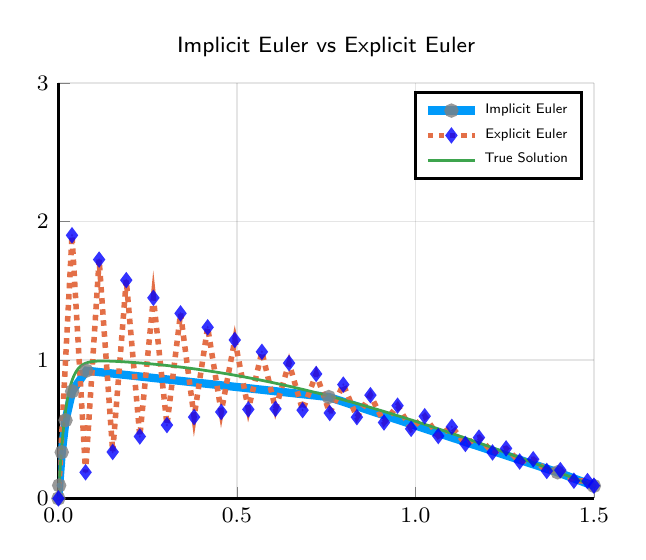
\begin{tikzpicture}[]
\begin{axis}[height = {68.58mm}, title = {Implicit Euler vs Explicit Euler}, xmin = {0.0}, xmax = {1.5}, ymax = {3}, unbounded coords=jump,scaled x ticks = false,xlabel style = {font = {\fontsize{11 pt}{14.3 pt}\selectfont}, color = {rgb,1:red,0.00000000;green,0.00000000;blue,0.00000000}, draw opacity = 1.0, rotate = 0.0},xmajorgrids = true,xtick = {0.0,0.5,1.0,1.5},xticklabels = {$0.0$,$0.5$,$1.0$,$1.5$},xtick align = inside,xticklabel style = {font = {\fontsize{8 pt}{10.4 pt}\selectfont}, color = {rgb,1:red,0.00000000;green,0.00000000;blue,0.00000000}, draw opacity = 1.0, rotate = 0.0},x grid style = {color = {rgb,1:red,0.00000000;green,0.00000000;blue,0.00000000},
draw opacity = 0.1,
line width = 0.5,
solid},axis lines* = left,x axis line style = {color = {rgb,1:red,0.00000000;green,0.00000000;blue,0.00000000},
draw opacity = 1.0,
line width = 1,
solid},scaled y ticks = false,ylabel style = {font = {\fontsize{11 pt}{14.3 pt}\selectfont}, color = {rgb,1:red,0.00000000;green,0.00000000;blue,0.00000000}, draw opacity = 1.0, rotate = 0.0},ymajorgrids = true,ytick = {0.0,1.0,2.0,3.0},yticklabels = {$0$,$1$,$2$,$3$},ytick align = inside,yticklabel style = {font = {\fontsize{8 pt}{10.4 pt}\selectfont}, color = {rgb,1:red,0.00000000;green,0.00000000;blue,0.00000000}, draw opacity = 1.0, rotate = 0.0},y grid style = {color = {rgb,1:red,0.00000000;green,0.00000000;blue,0.00000000},
draw opacity = 0.1,
line width = 0.5,
solid},axis lines* = left,y axis line style = {color = {rgb,1:red,0.00000000;green,0.00000000;blue,0.00000000},
draw opacity = 1.0,
line width = 1,
solid},    xshift = 0.0mm,
    yshift = 0.0mm,
    axis background/.style={fill={rgb,1:red,1.00000000;green,1.00000000;blue,1.00000000}}
,title style = {font = {\fontsize{8 pt}{10.4 pt}\selectfont}, color = {rgb,1:red,0.00000000;green,0.00000000;blue,0.00000000}, draw opacity = 1.0, rotate = 0.0},legend style = {color = {rgb,1:red,0.00000000;green,0.00000000;blue,0.00000000},
draw opacity = 1.0,
line width = 1,
solid,fill = {rgb,1:red,1.00000000;green,1.00000000;blue,1.00000000},font = {\fontsize{3 pt}{3.9000000000000004 pt}\selectfont}},colorbar style={title=}, ymin = {0}, width = {83.82000000000001mm}]\addplot+ [color = {rgb,1:red,0.00000000;green,0.60560316;blue,0.97868012},
draw opacity = 1.0,
line width = 3,
solid,mark = *,
mark size = 1.0,
mark options = {
    color = {rgb,1:red,0.50196078;green,0.50196078;blue,0.50196078}, draw opacity = 0.8,
    fill = {rgb,1:red,0.00000000;green,0.60560316;blue,0.97868012}, fill opacity = 0.8,
    line width = 3,
    rotate = 0,
    solid
}]coordinates {
(0.0, 0.0)
(0.0020771986833039288, 0.09408776139589611)
(0.009260326368768204, 0.3334632802663635)
(0.019877922742195877, 0.5645369467270349)
(0.03835984188506675, 0.7733258253168489)
(0.07836244363528605, 0.922399330030937)
(0.7572702195977378, 0.73231366137981)
(1.398145325945461, 0.188757474090256)
(1.5, 0.09010786156864856)
};
\addlegendentry{Implicit Euler}
\addplot+ [color = {rgb,1:red,0.88887350;green,0.43564919;blue,0.27812294},
draw opacity = 1.0,
line width = 2,
dotted,mark = diamond*,
mark size = 0.5,
mark options = {
    color = {rgb,1:red,0.00000000;green,0.00000000;blue,1.00000000}, draw opacity = 0.8,
    fill = {rgb,1:red,0.88887350;green,0.43564919;blue,0.27812294}, fill opacity = 0.8,
    line width = 3,
    rotate = 0,
    solid
}]coordinates {
(0.0, 0.0)
(0.038, 1.9)
(0.076, 0.18862836506532132)
(0.11399999999999999, 1.7247499121050163)
(0.152, 0.33539224424914066)
(0.19, 1.576240406400587)
(0.228, 0.44719168096228534)
(0.266, 1.4483562517249784)
(0.304, 0.5296565807577014)
(0.34199999999999997, 1.3361879379800254)
(0.37999999999999995, 0.5873938877499988)
(0.4179999999999999, 1.2358083086203704)
(0.4559999999999999, 0.6241875277868691)
(0.4939999999999999, 1.14409134692611)
(0.5319999999999999, 0.6431600604720726)
(0.57, 1.0585650754715115)
(0.608, 0.6469032848839504)
(0.646, 0.9772920577465439)
(0.684, 0.6375836692322051)
(0.7220000000000001, 0.8987722299892003)
(0.7600000000000001, 0.617027361433551)
(0.7980000000000002, 0.8218637951175238)
(0.8360000000000002, 0.586788635997346)
(0.8740000000000002, 0.745718723899805)
(0.9120000000000003, 0.5482049024647213)
(0.9500000000000003, 0.6697300673666756)
(0.9880000000000003, 0.5024408093513701)
(1.0260000000000002, 0.5934888182687575)
(1.0640000000000003, 0.45052349870827757)
(1.1020000000000003, 0.5167484918657174)
(1.1400000000000003, 0.3933706786542554)
(1.1780000000000004, 0.43939594673204996)
(1.2160000000000004, 0.33181286722919534)
(1.2540000000000004, 0.3614272501614598)
(1.2920000000000005, 0.26661090663781506)
(1.3300000000000005, 0.28292762276458283)
(1.3680000000000005, 0.19846964103594864)
(1.4060000000000006, 0.20405468320522818)
(1.4440000000000006, 0.1280484842496745)
(1.4820000000000007, 0.1250243649873216)
(1.5, 0.09231415098263084)
};
\addlegendentry{Explicit Euler}
\addplot+ [color = {rgb,1:red,0.24222430;green,0.64327509;blue,0.30444865},
draw opacity = 1.0,
line width = 1,
solid,mark = none,
mark size = 2.0,
mark options = {
    color = {rgb,1:red,0.00000000;green,0.00000000;blue,0.00000000}, draw opacity = 1.0,
    fill = {rgb,1:red,0.24222430;green,0.64327509;blue,0.30444865}, fill opacity = 1.0,
    line width = 1,
    rotate = 0,
    solid
}]coordinates {
(0.0, 0.0)
(0.0012831479897348161, 0.06214261302928963)
(0.0025662959794696323, 0.12042341776489711)
(0.003849443969204448, 0.17508229481643328)
(0.0051325919589392645, 0.22634421798179777)
(0.00641573994867408, 0.2744201805958292)
(0.007698887938408896, 0.31950806431318796)
(0.008982035928143712, 0.36179345390302386)
(0.010265183917878529, 0.4014504014095412)
(0.011548331907613344, 0.4386421428264258)
(0.01283147989734816, 0.473521770234656)
(0.014114627887082978, 0.506232862172282)
(0.015397775876817793, 0.5369100748307147)
(0.016680923866552608, 0.5656796965135071)
(0.017964071856287425, 0.5926601676388645)
(0.01924721984602224, 0.6179625684280043)
(0.020530367835757058, 0.641691076287347)
(0.021813515825491875, 0.6639433947678351)
(0.023096663815226688, 0.6848111558674433)
(0.024379811804961505, 0.7043802973336557)
(0.02566295979469632, 0.7227314165192537)
(0.02694610778443114, 0.7399401022487577)
(0.028229255774165955, 0.7560772460616776)
(0.02951240376390077, 0.7712093341143279)
(0.030795551753635585, 0.7853987209420771)
(0.0320786997433704, 0.7987038862093359)
(0.033361847733105215, 0.8111796755043799)
(0.034644995722840036, 0.8228775261706007)
(0.03592814371257485, 0.8338456791039001)
(0.03721129170230967, 0.8441293773887213)
(0.03849443969204448, 0.8537710525897122)
(0.039777587681779296, 0.8628104994675269)
(0.041060735671514116, 0.8712850398367353)
(0.04234388366124893, 0.8792296762413958)
(0.04362703165098375, 0.8866772360808706)
(0.04491017964071856, 0.8936585067789996)
(0.046193327630453376, 0.9002023625539413)
(0.0474764756201882, 0.9063358833098665)
(0.04875962360992301, 0.912084466140539)
(0.05004277159965783, 0.9174719299037447)
(0.05132591958939264, 0.9225206132971677)
(0.05260906757912746, 0.9272514668396689)
(0.05389221556886228, 0.9316841391364572)
(0.05517536355859709, 0.9358370577836602)
(0.05645851154833191, 0.9397275052451781)
(0.057741659538066724, 0.9433716900143886)
(0.05902480752780154, 0.9467848133536763)
(0.06030795551753636, 0.9499811318865334)
(0.06159110350727117, 0.952974016300144)
(0.06287425149700598, 0.9557760063999227)
(0.0641573994867408, 0.9583988627429114)
(0.06544054747647562, 0.9608536150624115)
(0.06672369546621043, 0.9631506076835007)
(0.06800684345594525, 0.965299542116328)
(0.06928999144568007, 0.967309517002379)
(0.07057313943541488, 0.9691890655785399)
(0.0718562874251497, 0.9709461908129807)
(0.07313943541488452, 0.9725883983577511)
(0.07442258340461934, 0.9741227274533524)
(0.07570573139435414, 0.9755557799128448)
(0.07698887938408897, 0.9768937473050593)
(0.07827202737382379, 0.97814243644849)
(0.07955517536355859, 0.9793072933206307)
(0.08083832335329341, 0.9803934254818968)
(0.08212147134302823, 0.981405623105909)
(0.08340461933276304, 0.9823483787029289)
(0.08468776732249786, 0.983225905617587)
(0.08597091531223268, 0.984042155377106)
(0.0872540633019675, 0.9848008339615204)
(0.0885372112917023, 0.9855054170628168)
(0.08982035928143713, 0.9861591643957555)
(0.09110350727117195, 0.9867651331194591)
(0.09238665526090675, 0.9873261904248697)
(0.09366980325064157, 0.9878450253401446)
(0.0949529512403764, 0.9883241598023706)
(0.0962360992301112, 0.9887659590410198)
(0.09751924721984602, 0.9891726413163396)
(0.09880239520958084, 0.9895462870527247)
(0.10008554319931566, 0.98988884740442)
(0.10136869118905047, 0.9902021522886811)
(0.10265183917878529, 0.9904879179198927)
(0.10393498716852011, 0.9907477538758105)
(0.10521813515825491, 0.9909831697242016)
(0.10650128314798973, 0.9911955812379523)
(0.10778443113772455, 0.991386316223885)
(0.10906757912745936, 0.9915566199893545)
(0.11035072711719418, 0.99170766046917)
(0.111633875106929, 0.9918405330339051)
(0.11291702309666382, 0.9919562649993694)
(0.11420017108639863, 0.9920558198558903)
(0.11548331907613345, 0.9921401012347629)
(0.11676646706586827, 0.9922099566281897)
(0.11804961505560307, 0.9922661808781719)
(0.1193327630453379, 0.992309519448454)
(0.12061591103507271, 0.9923406714931227)
(0.12189905902480752, 0.992360292734581)
(0.12318220701454234, 0.9923689981627276)
(0.12446535500427716, 0.9923673645663849)
(0.12574850299401197, 0.9923559329073474)
(0.1270316509837468, 0.9923352105468549)
(0.1283147989734816, 0.9923056733338199)
(0.12959794696321641, 0.9922677675633789)
(0.13088109495295125, 0.9922219118134966)
(0.13216424294268606, 0.9921684986675312)
(0.13344739093242086, 0.992107896329806)
(0.1347305389221557, 0.9920404501407939)
(0.1360136869118905, 0.9919664839980942)
(0.1372968349016253, 0.9918863016890767)
(0.13857998289136014, 0.9918001881407331)
(0.13986313088109495, 0.9917084105919172)
(0.14114627887082976, 0.9916112196927449)
(0.1424294268605646, 0.9915088505355404)
(0.1437125748502994, 0.9914015236218615)
(0.14499572284003423, 0.9912894457693588)
(0.14627887082976904, 0.991172810962214)
(0.14756201881950384, 0.9910518011489057)
(0.14884516680923868, 0.9909265869903682)
(0.15012831479897348, 0.9907973285615519)
(0.1514114627887083, 0.9906641760093464)
(0.15269461077844312, 0.9905272701696901)
(0.15397775876817793, 0.9903867431464424)
(0.15526090675791274, 0.9902427188542581)
(0.15654405474764757, 0.9900953135274534)
(0.15782720273738238, 0.9899446361975576)
(0.15911035072711718, 0.9897907891410636)
(0.16039349871685202, 0.98963386829929)
(0.16167664670658682, 0.9894739636723469)
(0.16295979469632163, 0.9893111596885498)
(0.16424294268605646, 0.9891455355507646)
(0.16552609067579127, 0.9889771655612122)
(0.16680923866552608, 0.9888061194261929)
(0.1680923866552609, 0.9886324625419838)
(0.16937553464499572, 0.9884562562628364)
(0.17065868263473055, 0.988277558152133)
(0.17194183062446536, 0.9880964222183287)
(0.17322497861420016, 0.9879128991358749)
(0.174508126603935, 0.9877270364525831)
(0.1757912745936698, 0.9875388787842225)
(0.1770744225834046, 0.9873484679969008)
(0.17835757057313945, 0.9871558433780016)
(0.17964071856287425, 0.9869610417965181)
(0.18092386655260906, 0.9867640978535702)
(0.1822070145423439, 0.9865650440236505)
(0.1834901625320787, 0.9863639107868565)
(0.1847733105218135, 0.9861607267528397)
(0.18605645851154834, 0.9859555187774195)
(0.18733960650128315, 0.9857483120715446)
(0.18862275449101795, 0.9855391303037471)
(0.1899059024807528, 0.9853279956962773)
(0.1911890504704876, 0.9851149291151242)
(0.1924721984602224, 0.9848999501543519)
(0.19375534644995723, 0.9846830772152491)
(0.19503849443969204, 0.9844643275807187)
(0.19632164242942687, 0.9842437174850739)
(0.19760479041916168, 0.9840212621791872)
(0.1988879384088965, 0.9837969759917536)
(0.20017108639863132, 0.9835708723868797)
(0.20145423438836613, 0.9833429640177994)
(0.20273738237810093, 0.9831132627775535)
(0.20402053036783577, 0.982881779846493)
(0.20530367835757057, 0.9826485257366807)
(0.20658682634730538, 0.9824135103334666)
(0.20786997433704021, 0.9821767429345694)
(0.20915312232677502, 0.98193823228689)
(0.21043627031650983, 0.9816979866210238)
(0.21171941830624466, 0.9814560136832327)
(0.21300256629597947, 0.9812123207658484)
(0.21428571428571427, 0.9809669147356351)
(0.2155688622754491, 0.9807198020602845)
(0.21685201026518391, 0.9804709888335212)
(0.21813515825491872, 0.9802204807985803)
(0.21941830624465355, 0.9799682833700762)
(0.22070145423438836, 0.979714401654475)
(0.2219846022241232, 0.9794588404694085)
(0.223267750213858, 0.9792016043619376)
(0.2245508982035928, 0.9789426976255989)
(0.22583404619332764, 0.9786821243160343)
(0.22711719418306245, 0.9784198882661524)
(0.22840034217279725, 0.9781559931000409)
(0.2296834901625321, 0.9778904422460444)
(0.2309666381522669, 0.9776232389492469)
(0.2322497861420017, 0.9773543862830704)
(0.23353293413173654, 0.977083887160011)
(0.23481608212147134, 0.9768117443416976)
(0.23609923011120615, 0.9765379604484585)
(0.23738237810094098, 0.9762625379684385)
(0.2386655260906758, 0.9759854792659781)
(0.2399486740804106, 0.9757067865891897)
(0.24123182207014543, 0.9754264620776228)
(0.24251497005988024, 0.9751445077689976)
(0.24379811804961504, 0.9748609256056966)
(0.24508126603934988, 0.974575717441003)
(0.24636441402908468, 0.9742888850448227)
(0.24764756201881952, 0.9740004301089206)
(0.24893071000855432, 0.9737103542518466)
(0.25021385799828916, 0.9734186590237048)
(0.25149700598802394, 0.9731253459107387)
(0.25278015397775877, 0.9728304163394143)
(0.2540633019674936, 0.9725338716800563)
(0.2553464499572284, 0.9722357132507836)
(0.2566295979469632, 0.9719359423207002)
(0.25791274593669805, 0.9716345601131557)
(0.25919589392643283, 0.9713315678088932)
(0.26047904191616766, 0.9710269665488568)
(0.2617621899059025, 0.9707207574367116)
(0.2630453378956373, 0.9704129415412437)
(0.2643284858853721, 0.9701035198987704)
(0.26561163387510695, 0.9697924935154928)
(0.2668947818648417, 0.9694798633694018)
(0.26817792985457656, 0.9691656304120433)
(0.2694610778443114, 0.9688497955705623)
(0.27074422583404617, 0.9685323597491606)
(0.272027373823781, 0.9682133238307732)
(0.27331052181351584, 0.9678926886786815)
(0.2745936698032506, 0.9675704551378728)
(0.27587681779298545, 0.9672466240362183)
(0.2771599657827203, 0.9669211961856357)
(0.27844311377245506, 0.9665941723833472)
(0.2797262617621899, 0.9662655534131085)
(0.28100940975192473, 0.9659353400460294)
(0.2822925577416595, 0.9656035330414586)
(0.28357570573139435, 0.965270133148047)
(0.2848588537211292, 0.9649351411043715)
(0.286142001710864, 0.9645985576398391)
(0.2874251497005988, 0.9642603834755328)
(0.2887082976903336, 0.963920619324846)
(0.28999144568006846, 0.9635792658939996)
(0.29127459366980324, 0.9632363238826037)
(0.2925577416595381, 0.9628917939843555)
(0.2938408896492729, 0.962545676887698)
(0.2951240376390077, 0.9621979732760942)
(0.2964071856287425, 0.9618486838285017)
(0.29769033361847735, 0.961497809219933)
(0.29897348160821213, 0.9611453501216776)
(0.30025662959794697, 0.9607913072018311)
(0.3015397775876818, 0.9604356811257532)
(0.3028229255774166, 0.9600784725563376)
(0.3041060735671514, 0.9597196821542037)
(0.30538922155688625, 0.9593593105779741)
(0.306672369546621, 0.958997358484697)
(0.30795551753635586, 0.9586338265302218)
(0.3092386655260907, 0.9582687153691475)
(0.3105218135158255, 0.9579020256552142)
(0.3118049615055603, 0.9575337580414971)
(0.31308810949529514, 0.9571639131804913)
(0.3143712574850299, 0.9567924917244524)
(0.31565440547476475, 0.9564194943256509)
(0.3169375534644996, 0.9560449216364579)
(0.31822070145423437, 0.9556687743093805)
(0.3195038494439692, 0.9552910529972035)
(0.32078699743370404, 0.9549117583532845)
(0.3220701454234388, 0.9545308910317662)
(0.32335329341317365, 0.9541484516873942)
(0.3246364414029085, 0.9537644409758202)
(0.32591958939264326, 0.9533788595536613)
(0.3272027373823781, 0.9529917080784994)
(0.32848588537211293, 0.9526029872091364)
(0.3297690333618477, 0.9522126976057399)
(0.33105218135158254, 0.9518208399298317)
(0.3323353293413174, 0.9514274148442495)
(0.33361847733105215, 0.951032423013233)
(0.334901625320787, 0.9506358651026633)
(0.3361847733105218, 0.9502377417801525)
(0.33746792130025666, 0.9498380537148357)
(0.33875106928999144, 0.9494368015776321)
(0.34003421727972627, 0.9490339860412026)
(0.3413173652694611, 0.9486296077799417)
(0.3426005132591959, 0.9482236674701837)
(0.3438836612489307, 0.9478161657902868)
(0.34516680923866555, 0.947407103420569)
(0.34644995722840033, 0.9469964810432386)
(0.34773310521813516, 0.9465842993424588)
(0.34901625320787, 0.9461705590045657)
(0.3502994011976048, 0.945755260718084)
(0.3515825491873396, 0.9453384051734882)
(0.35286569717707444, 0.9449199930634873)
(0.3541488451668092, 0.944500025082894)
(0.35543199315654406, 0.9440785019286356)
(0.3567151411462789, 0.9436554242999335)
(0.35799828913601367, 0.9432307928983473)
(0.3592814371257485, 0.9428046084276829)
(0.36056458511548334, 0.9423768715939111)
(0.3618477331052181, 0.9419475831052376)
(0.36313088109495295, 0.9415167436722903)
(0.3644140290846878, 0.9410843540081025)
(0.36569717707442256, 0.9406504148278625)
(0.3669803250641574, 0.9402149268492108)
(0.36826347305389223, 0.9397778907920561)
(0.369546621043627, 0.939339307378611)
(0.37082976903336184, 0.938899177333555)
(0.3721129170230967, 0.9384575013840497)
(0.37339606501283146, 0.938014280259631)
(0.3746792130025663, 0.9375695146921306)
(0.3759623609923011, 0.9371232054157494)
(0.3772455089820359, 0.9366753531672333)
(0.37852865697177074, 0.9362259586858301)
(0.3798118049615056, 0.9357750227130247)
(0.38109495295124035, 0.9353225459928681)
(0.3823781009409752, 0.9348685292717438)
(0.38366124893071, 0.9344129732984346)
(0.3849443969204448, 0.933955878824271)
(0.38622754491017963, 0.9334972466031257)
(0.38751069289991447, 0.9330370773912967)
(0.3887938408896493, 0.9325753719474347)
(0.3900769888793841, 0.9321121310326206)
(0.3913601368691189, 0.9316473554105666)
(0.39264328485885375, 0.9311810458474514)
(0.3939264328485885, 0.9307132031118024)
(0.39520958083832336, 0.9302438279747198)
(0.3964927288280582, 0.929772921209666)
(0.397775876817793, 0.9293004835925507)
(0.3990590248075278, 0.9288265159018656)
(0.40034217279726264, 0.9283510189186625)
(0.4016253207869974, 0.9278739934264332)
(0.40290846877673225, 0.9273954402110369)
(0.4041916167664671, 0.9269153600608092)
(0.40547476475620187, 0.9264337537667312)
(0.4067579127459367, 0.9259506221222322)
(0.40804106073567153, 0.9254659659231397)
(0.4093242087254063, 0.9249797859678455)
(0.41060735671514115, 0.9244920830571093)
(0.411890504704876, 0.9240028579941615)
(0.41317365269461076, 0.9235121115848265)
(0.4144568006843456, 0.923019844637484)
(0.41573994867408043, 0.9225260579629468)
(0.4170230966638152, 0.9220307523744047)
(0.41830624465355004, 0.9215339286875351)
(0.4195893926432849, 0.9210355877206641)
(0.42087254063301965, 0.9205357302945542)
(0.4221556886227545, 0.9200343572323636)
(0.4234388366124893, 0.9195314693598168)
(0.4247219846022241, 0.9190270675049962)
(0.42600513259195893, 0.9185211524984656)
(0.42728828058169377, 0.9180137251733805)
(0.42857142857142855, 0.9175047863654384)
(0.4298545765611634, 0.916994336912755)
(0.4311377245508982, 0.9164823776558182)
(0.432420872540633, 0.9159689094376158)
(0.43370402053036783, 0.915453933103778)
(0.43498716852010266, 0.9149374495023145)
(0.43627031650983744, 0.9144194594836875)
(0.4375534644995723, 0.9138999639008736)
(0.4388366124893071, 0.9133789636092042)
(0.44011976047904194, 0.9128564594664965)
(0.4414029084687767, 0.912332452333151)
(0.44268605645851156, 0.9118069430720893)
(0.4439692044482464, 0.9112799325486325)
(0.44525235243798117, 0.9107514216304667)
(0.446535500427716, 0.9102214111877854)
(0.44781864841745084, 0.9096899020933994)
(0.4491017964071856, 0.9091568952224741)
(0.45038494439692045, 0.9086223914526391)
(0.4516680923866553, 0.9080863916640043)
(0.45295124037639006, 0.9075488967390268)
(0.4542343883661249, 0.9070099075626481)
(0.45551753635585973, 0.9064694250223797)
(0.4568006843455945, 0.9059274500082335)
(0.45808383233532934, 0.9053839834125977)
(0.4593669803250642, 0.9048390261302144)
(0.46065012831479896, 0.9042925790583379)
(0.4619332763045338, 0.9037446430968217)
(0.4632164242942686, 0.9031952191478442)
(0.4644995722840034, 0.9026443081160362)
(0.46578272027373824, 0.9020919109084966)
(0.46706586826347307, 0.9015380284346549)
(0.46834901625320785, 0.9009826616064217)
(0.4696321642429427, 0.9004258113382619)
(0.4709153122326775, 0.8998674785471157)
(0.4721984602224123, 0.8993076641522787)
(0.47348160821214713, 0.8987463690753937)
(0.47476475620188197, 0.8981835942406057)
(0.47604790419161674, 0.8976193405746491)
(0.4773310521813516, 0.897053609006534)
(0.4786142001710864, 0.8964864004677437)
(0.4798973481608212, 0.8959177158921893)
(0.481180496150556, 0.8953475562161034)
(0.48246364414029086, 0.8947759223781948)
(0.48374679213002564, 0.8942028153197081)
(0.48502994011976047, 0.8936282359843383)
(0.4863130881094953, 0.8930521853181138)
(0.4875962360992301, 0.8924746642694024)
(0.4888793840889649, 0.8918956737890675)
(0.49016253207869975, 0.8913152148305283)
(0.4914456800684346, 0.8907332883494705)
(0.49272882805816937, 0.8901498953040414)
(0.4940119760479042, 0.8895650366547837)
(0.49529512403763903, 0.8889787133645539)
(0.4965782720273738, 0.8883909263986761)
(0.49786142001710865, 0.8878016767249911)
(0.4991445680068435, 0.8872109653137652)
(0.5004277159965783, 0.8866187931375746)
(0.501710863986313, 0.8860251611713258)
(0.5029940119760479, 0.8854300703924174)
(0.5042771599657827, 0.8848335217807768)
(0.5055603079555175, 0.8842355163185611)
(0.5068434559452524, 0.8836360549903999)
(0.5081266039349872, 0.8830351387832797)
(0.5094097519247219, 0.882432768686492)
(0.5106928999144568, 0.8818289456917864)
(0.5119760479041916, 0.8812236707934094)
(0.5132591958939264, 0.880616944988005)
(0.5145423438836613, 0.8800087692745077)
(0.5158254918733961, 0.8793991446541752)
(0.5171086398631308, 0.8787880721307434)
(0.5183917878528657, 0.8781755527104467)
(0.5196749358426005, 0.8775615874017324)
(0.5209580838323353, 0.8769461772155118)
(0.5222412318220702, 0.8763293231650208)
(0.523524379811805, 0.8757110262657909)
(0.5248075278015398, 0.8750912875358005)
(0.5260906757912746, 0.8744701079955043)
(0.5273738237810094, 0.873847488667727)
(0.5286569717707442, 0.8732234305775638)
(0.5299401197604791, 0.872597934752421)
(0.5312232677502139, 0.8719710022221749)
(0.5325064157399487, 0.8713426340191746)
(0.5337895637296834, 0.870712831177949)
(0.5350727117194183, 0.8700815947354922)
(0.5363558597091531, 0.8694489257310889)
(0.537639007698888, 0.8688148252063096)
(0.5389221556886228, 0.8681792942051595)
(0.5402053036783576, 0.867542333774096)
(0.5414884516680923, 0.8669039449619228)
(0.5427715996578272, 0.866264128819695)
(0.544054747647562, 0.8656228864007598)
(0.5453378956372968, 0.8649802187609428)
(0.5466210436270317, 0.864336126958466)
(0.5479041916167665, 0.8636906120537695)
(0.5491873396065012, 0.8630436751097125)
(0.5504704875962361, 0.8623953171914218)
(0.5517536355859709, 0.8617455393663007)
(0.5530367835757057, 0.8610943427041721)
(0.5543199315654406, 0.8604417282772892)
(0.5556030795551754, 0.859787697160226)
(0.5568862275449101, 0.8591322504297831)
(0.558169375534645, 0.8584753891650525)
(0.5594525235243798, 0.8578171144475616)
(0.5607356715141146, 0.8571574273612624)
(0.5620188195038495, 0.8564963289922393)
(0.5633019674935843, 0.8558338204290203)
(0.564585115483319, 0.8551699027623644)
(0.5658682634730539, 0.8545045770852945)
(0.5671514114627887, 0.8538378444932385)
(0.5684345594525235, 0.8531697060840313)
(0.5697177074422584, 0.8525001629578006)
(0.5710008554319932, 0.8518292162168865)
(0.572284003421728, 0.8511568669658915)
(0.5735671514114628, 0.8504831163118775)
(0.5748502994011976, 0.8498079653642381)
(0.5761334473909324, 0.8491314152345389)
(0.5774165953806673, 0.848453467036745)
(0.5786997433704021, 0.84777412188703)
(0.5799828913601369, 0.8470933809038204)
(0.5812660393498716, 0.8464112452079297)
(0.5825491873396065, 0.8457277159225549)
(0.5838323353293413, 0.8450427941731601)
(0.5851154833190761, 0.8443564810874006)
(0.586398631308811, 0.8436687777951904)
(0.5876817792985458, 0.8429796854288628)
(0.5889649272882805, 0.8422892051230727)
(0.5902480752780154, 0.8415973380146277)
(0.5915312232677502, 0.8409040852427102)
(0.592814371257485, 0.8402094479486877)
(0.5940975192472199, 0.8395134272761664)
(0.5953806672369547, 0.8388160243711225)
(0.5966638152266894, 0.8381172403818906)
(0.5979469632164243, 0.837417076459048)
(0.5992301112061591, 0.8367155337553422)
(0.6005132591958939, 0.836012613425764)
(0.6017964071856288, 0.8353083166277049)
(0.6030795551753636, 0.834602644520854)
(0.6043627031650983, 0.8338955982670274)
(0.6056458511548332, 0.8331871790304012)
(0.606928999144568, 0.8324773879773096)
(0.6082121471343028, 0.8317662262763114)
(0.6094952951240377, 0.8310536950983158)
(0.6107784431137725, 0.8303397956165667)
(0.6120615911035072, 0.8296245290065248)
(0.613344739093242, 0.8289078964457995)
(0.6146278870829769, 0.8281898991142266)
(0.6159110350727117, 0.8274705381940431)
(0.6171941830624466, 0.8267498148697151)
(0.6184773310521814, 0.8260277303278492)
(0.6197604790419161, 0.8253042857573807)
(0.621043627031651, 0.8245794823493794)
(0.6223267750213858, 0.8238533212971234)
(0.6236099230111206, 0.8231258037962216)
(0.6248930710008554, 0.822396931044592)
(0.6261762189905903, 0.821666704242348)
(0.6274593669803251, 0.8209351245917234)
(0.6287425149700598, 0.8202021932971766)
(0.6300256629597947, 0.8194679115655191)
(0.6313088109495295, 0.8187322806057905)
(0.6325919589392643, 0.8179953016291448)
(0.6338751069289992, 0.8172569758490374)
(0.635158254918734, 0.8165173044810371)
(0.6364414029084687, 0.8157762887429033)
(0.6377245508982036, 0.815033929854706)
(0.6390076988879384, 0.8142902290387986)
(0.6402908468776732, 0.8135451875197057)
(0.6415739948674081, 0.8127988065240541)
(0.6428571428571429, 0.8120510872806687)
(0.6441402908468776, 0.8113020310207097)
(0.6454234388366125, 0.8105516389775596)
(0.6467065868263473, 0.8097999123866536)
(0.6479897348160821, 0.8090468524857363)
(0.649272882805817, 0.8082924605146332)
(0.6505560307955518, 0.8075367377153431)
(0.6518391787852865, 0.8067796853321528)
(0.6531223267750214, 0.8060213046116087)
(0.6544054747647562, 0.805261596802401)
(0.655688622754491, 0.804500563155305)
(0.6569717707442259, 0.8037382049232698)
(0.6582549187339607, 0.802974523361583)
(0.6595380667236954, 0.8022095197276503)
(0.6608212147134302, 0.8014431952810142)
(0.6621043627031651, 0.8006755512834381)
(0.6633875106928999, 0.7999065889987587)
(0.6646706586826348, 0.7991363096929653)
(0.6659538066723696, 0.7983647146343137)
(0.6672369546621043, 0.7975918050932945)
(0.6685201026518391, 0.7968175823425171)
(0.669803250641574, 0.7960420476566569)
(0.6710863986313088, 0.7952652023125379)
(0.6723695466210436, 0.7944870475892829)
(0.6736526946107785, 0.7937075847681646)
(0.6749358426005133, 0.7929268151325047)
(0.676218990590248, 0.7921447399678565)
(0.6775021385799829, 0.7913613605618157)
(0.6787852865697177, 0.790576678204111)
(0.6800684345594525, 0.7897906941867131)
(0.6813515825491874, 0.7890034098038029)
(0.6826347305389222, 0.788214826351657)
(0.6839178785286569, 0.7874249451285917)
(0.6852010265183918, 0.7866337674350619)
(0.6864841745081266, 0.7858412945737822)
(0.6877673224978614, 0.7850475278495955)
(0.6890504704875963, 0.78425246856938)
(0.6903336184773311, 0.7834561180422144)
(0.6916167664670658, 0.7826584775791983)
(0.6928999144568007, 0.7818595484935413)
(0.6941830624465355, 0.7810593321006719)
(0.6954662104362703, 0.7802578297182036)
(0.6967493584260052, 0.7794550426658207)
(0.69803250641574, 0.7786509722652278)
(0.6993156544054747, 0.7778456198402344)
(0.7005988023952096, 0.7770389867169)
(0.7018819503849444, 0.7762310742233989)
(0.7031650983746792, 0.7754218836898705)
(0.704448246364414, 0.7746114164486719)
(0.7057313943541489, 0.7737996738341454)
(0.7070145423438836, 0.7729866571827202)
(0.7082976903336184, 0.7721723678330192)
(0.7095808383233533, 0.7713568071258263)
(0.7108639863130881, 0.770539976403973)
(0.712147134302823, 0.769721877012285)
(0.7134302822925578, 0.7689025102976701)
(0.7147134302822925, 0.7680818776092735)
(0.7159965782720273, 0.7672599802982905)
(0.7172797262617622, 0.7664368197179121)
(0.718562874251497, 0.7656123972234882)
(0.7198460222412318, 0.7647867141723389)
(0.7211291702309667, 0.7639597719238459)
(0.7224123182207014, 0.76313157183956)
(0.7236954662104362, 0.7623021152831682)
(0.7249786142001711, 0.7614714036203794)
(0.7262617621899059, 0.7606394382188771)
(0.7275449101796407, 0.7598062204483965)
(0.7288280581693756, 0.7589717516808924)
(0.7301112061591104, 0.7581360332903357)
(0.7313943541488451, 0.7572990666526747)
(0.73267750213858, 0.7564608531459905)
(0.7339606501283148, 0.7556213941503114)
(0.7352437981180496, 0.7547806910477005)
(0.7365269461077845, 0.7539387452223643)
(0.7378100940975193, 0.753095558060621)
(0.739093242087254, 0.7522511309507868)
(0.7403763900769889, 0.7514054652831315)
(0.7416595380667237, 0.7505585624499485)
(0.7429426860564585, 0.7497104238457071)
(0.7442258340461934, 0.7488610508669012)
(0.7455089820359282, 0.7480104449119592)
(0.7467921300256629, 0.7471586073814174)
(0.7480752780153977, 0.746305539677737)
(0.7493584260051326, 0.7454512432053875)
(0.7506415739948674, 0.7445957193709543)
(0.7519247219846023, 0.74373896958311)
(0.7532078699743371, 0.742880995252507)
(0.7544910179640718, 0.7420217977917154)
(0.7557741659538066, 0.7411613786153041)
(0.7570573139435415, 0.7402997391400119)
(0.7583404619332763, 0.7394368807845406)
(0.7596236099230111, 0.7385728049695364)
(0.760906757912746, 0.7377075131177091)
(0.7621899059024807, 0.736841006653675)
(0.7634730538922155, 0.735973287004029)
(0.7647562018819504, 0.735104355597455)
(0.7660393498716852, 0.7342342138646994)
(0.76732249786142, 0.7333628632384676)
(0.7686056458511549, 0.7324903051533477)
(0.7698887938408896, 0.7316165410459244)
(0.7711719418306244, 0.730741572354883)
(0.7724550898203593, 0.729865400520885)
(0.7737382378100941, 0.7289880269864949)
(0.7750213857998289, 0.7281094531963167)
(0.7763045337895638, 0.727229680596838)
(0.7775876817792986, 0.7263487106364953)
(0.7788708297690333, 0.7254665447657855)
(0.7801539777587682, 0.7245831844372443)
(0.781437125748503, 0.7236986311053405)
(0.7827202737382378, 0.7228128862264094)
(0.7840034217279727, 0.7219259512587357)
(0.7852865697177075, 0.7210378276626908)
(0.7865697177074422, 0.7201485169006135)
(0.787852865697177, 0.7192580204366777)
(0.7891360136869119, 0.7183663397371028)
(0.7904191616766467, 0.7174734762699606)
(0.7917023096663816, 0.7165794315052402)
(0.7929854576561164, 0.7156842069149616)
(0.7942686056458511, 0.7147878039731603)
(0.795551753635586, 0.7138902241557818)
(0.7968349016253208, 0.7129914689406129)
(0.7981180496150556, 0.7120915398073596)
(0.7994011976047904, 0.711190438237773)
(0.8006843455945253, 0.7102881657155765)
(0.80196749358426, 0.7093847237262777)
(0.8032506415739948, 0.7084801137574112)
(0.8045337895637297, 0.7075743372983413)
(0.8058169375534645, 0.706667395840317)
(0.8071000855431993, 0.7057592908765876)
(0.8083832335329342, 0.7048500239023933)
(0.8096663815226689, 0.703939596414863)
(0.8109495295124037, 0.7030280099129436)
(0.8122326775021386, 0.7021152658974594)
(0.8135158254918734, 0.7012013658712776)
(0.8147989734816082, 0.7002863113391486)
(0.8160821214713431, 0.6993701038076693)
(0.8173652694610778, 0.6984527447853777)
(0.8186484174508126, 0.6975342357826346)
(0.8199315654405475, 0.6966145783116516)
(0.8212147134302823, 0.6956937738866099)
(0.8224978614200171, 0.6947718240236556)
(0.823781009409752, 0.6938487302408043)
(0.8250641573994867, 0.6929244940578624)
(0.8263473053892215, 0.6919991169964799)
(0.8276304533789564, 0.6910726005803047)
(0.8289136013686912, 0.6901449463348867)
(0.830196749358426, 0.6892161557875535)
(0.8314798973481609, 0.6882862304675619)
(0.8327630453378957, 0.6873551719059698)
(0.8340461933276304, 0.6864229816356506)
(0.8353293413173652, 0.6854896611914134)
(0.8366124893071001, 0.6845552121100096)
(0.8378956372968349, 0.6836196359300367)
(0.8391787852865698, 0.6826829341918619)
(0.8404619332763046, 0.6817451084376477)
(0.8417450812660393, 0.6808061602115476)
(0.8430282292557741, 0.6798660910595735)
(0.844311377245509, 0.6789249025294941)
(0.8455945252352438, 0.6779825961709783)
(0.8468776732249786, 0.6770391735354773)
(0.8481608212147135, 0.6760946361762203)
(0.8494439692044482, 0.6751489856483397)
(0.850727117194183, 0.674202223508884)
(0.8520102651839179, 0.6732543513167293)
(0.8532934131736527, 0.6723053706324881)
(0.8545765611633875, 0.6713552830185545)
(0.8558597091531224, 0.6704040900392165)
(0.8571428571428571, 0.6694517932607225)
(0.8584260051325919, 0.6684983942509235)
(0.8597091531223268, 0.6675438945796025)
(0.8609923011120616, 0.6665882958182955)
(0.8622754491017964, 0.6656315995402798)
(0.8635585970915313, 0.6646738073206994)
(0.864841745081266, 0.6637149207365898)
(0.8661248930710008, 0.6627549413667898)
(0.8674080410607357, 0.6617938707918632)
(0.8686911890504705, 0.6608317105940955)
(0.8699743370402053, 0.659868462357658)
(0.8712574850299402, 0.6589041276686272)
(0.8725406330196749, 0.6579387081147002)
(0.8738237810094097, 0.6569722052854375)
(0.8751069289991446, 0.6560046207721484)
(0.8763900769888794, 0.6550359561678453)
(0.8776732249786142, 0.6540662130673697)
(0.878956372968349, 0.6530953930674286)
(0.8802395209580839, 0.6521234977665125)
(0.8815226689478186, 0.6511505287648098)
(0.8828058169375534, 0.6501764876641972)
(0.8840889649272883, 0.6492013760684175)
(0.8853721129170231, 0.6482251955830349)
(0.886655260906758, 0.647247947815297)
(0.8879384088964928, 0.6462696343742185)
(0.8892215568862275, 0.6452902568705651)
(0.8905047048759623, 0.6443098169167686)
(0.8917878528656972, 0.6433283161270501)
(0.893071000855432, 0.6423457561174676)
(0.8943541488451668, 0.6413621385058466)
(0.8956372968349017, 0.6403774649116791)
(0.8969204448246364, 0.6393917369561279)
(0.8982035928143712, 0.6384049562621487)
(0.8994867408041061, 0.6374171244545265)
(0.9007698887938409, 0.6364282431597049)
(0.9020530367835757, 0.6354383140058393)
(0.9033361847733106, 0.6344473386228319)
(0.9046193327630453, 0.6334553186422143)
(0.9059024807527801, 0.632462255697265)
(0.907185628742515, 0.6314681514230712)
(0.9084687767322498, 0.6304730074564662)
(0.9097519247219846, 0.6294768254359293)
(0.9110350727117195, 0.6284796070015795)
(0.9123182207014542, 0.6274813537952697)
(0.913601368691189, 0.6264820674606976)
(0.9148845166809239, 0.6254817496431333)
(0.9161676646706587, 0.6244804019895853)
(0.9174508126603935, 0.6234780261487569)
(0.9187339606501284, 0.622474623770956)
(0.9200171086398631, 0.6214701965081941)
(0.9213002566295979, 0.6204647460142593)
(0.9225834046193327, 0.6194582739446669)
(0.9238665526090676, 0.6184507819565622)
(0.9251497005988024, 0.6174422717086867)
(0.9264328485885372, 0.6164327448614804)
(0.927715996578272, 0.6154222030771525)
(0.9289991445680068, 0.6144106480195944)
(0.9302822925577416, 0.6133980813542558)
(0.9315654405474765, 0.6123845047483315)
(0.9328485885372113, 0.6113699198705795)
(0.9341317365269461, 0.6103543283914156)
(0.935414884516681, 0.6093377319829985)
(0.9366980325064157, 0.6083201323191951)
(0.9379811804961505, 0.6073015310754799)
(0.9392643284858854, 0.6062819299288951)
(0.9405474764756202, 0.6052613305581271)
(0.941830624465355, 0.6042397346436288)
(0.9431137724550899, 0.6032171438674542)
(0.9443969204448246, 0.6021935599132618)
(0.9456800684345594, 0.6011689844663766)
(0.9469632164242943, 0.6001434192136765)
(0.9482463644140291, 0.5991168658436499)
(0.9495295124037639, 0.5980893260464918)
(0.9508126603934988, 0.5970608015140831)
(0.9520958083832335, 0.5960312939399003)
(0.9533789563729683, 0.5950008050189456)
(0.9546621043627032, 0.5939693364478338)
(0.955945252352438, 0.5929368899248753)
(0.9572284003421728, 0.5919034671500383)
(0.9585115483319077, 0.5908690698247875)
(0.9597946963216424, 0.5898336996522588)
(0.9610778443113772, 0.588797358337117)
(0.962360992301112, 0.5877600475855883)
(0.9636441402908469, 0.5867217691055658)
(0.9649272882805817, 0.5856825246066073)
(0.9662104362703166, 0.5846423157998474)
(0.9674935842600513, 0.5836011443979231)
(0.9687767322497861, 0.5825590121150211)
(0.9700598802395209, 0.5815159206670093)
(0.9713430282292558, 0.5804718717713805)
(0.9726261762189906, 0.5794268671471006)
(0.9739093242087254, 0.5783809085147646)
(0.9751924721984602, 0.577333997596488)
(0.976475620188195, 0.5762861361158965)
(0.9777587681779298, 0.5752373257982412)
(0.9790419161676647, 0.5741875683704132)
(0.9803250641573995, 0.5731368655608629)
(0.9816082121471343, 0.5720852190995194)
(0.9828913601368692, 0.571032630717816)
(0.9841745081266039, 0.5699791021488111)
(0.9854576561163387, 0.5689246351272004)
(0.9867408041060736, 0.567869231389101)
(0.9880239520958084, 0.5668128926722215)
(0.9893071000855432, 0.5657556207157858)
(0.9905902480752781, 0.564697417260481)
(0.9918733960650128, 0.5636382840485709)
(0.9931565440547476, 0.5625782228239327)
(0.9944396920444825, 0.5615172353319878)
(0.9957228400342173, 0.5604553233196158)
(0.9970059880239521, 0.5593924885351502)
(0.998289136013687, 0.5583287327285097)
(0.9995722840034217, 0.5572640576512037)
(1.0008554319931566, 0.5561984650561996)
(1.0021385799828915, 0.5551319566979548)
(1.003421727972626, 0.5540645343324564)
(1.004704875962361, 0.5529961997171086)
(1.0059880239520957, 0.5519269546108421)
(1.0072711719418306, 0.5508568007741713)
(1.0085543199315654, 0.5497857399691373)
(1.0098374679213002, 0.5487137739592216)
(1.011120615911035, 0.5476409045093202)
(1.01240376390077, 0.5465671333858382)
(1.0136869118905047, 0.5454924623567907)
(1.0149700598802396, 0.5444168931916137)
(1.0162532078699744, 0.5433404276611729)
(1.0175363558597093, 0.5422630675378651)
(1.0188195038494439, 0.5411848145954681)
(1.0201026518391787, 0.5401056706092302)
(1.0213857998289135, 0.5390256373559479)
(1.0226689478186484, 0.5379447166139311)
(1.0239520958083832, 0.536862910162907)
(1.025235243798118, 0.5357802197839885)
(1.0265183917878529, 0.5346966472597349)
(1.0278015397775877, 0.5336121943742795)
(1.0290846877673225, 0.532526862913173)
(1.0303678357570574, 0.5314406546633683)
(1.0316509837467922, 0.5303535714132998)
(1.032934131736527, 0.529265614952769)
(1.0342172797262617, 0.5281767870729924)
(1.0355004277159965, 0.5270870895666931)
(1.0367835757057313, 0.5259965242280875)
(1.0380667236954662, 0.524905092852801)
(1.039349871685201, 0.5238127972378019)
(1.0406330196749358, 0.5227196391814588)
(1.0419161676646707, 0.5216256204836456)
(1.0431993156544055, 0.5205307429457289)
(1.0444824636441403, 0.5194350083703325)
(1.0457656116338752, 0.5183384185615871)
(1.04704875962361, 0.5172409753249672)
(1.0483319076133448, 0.5161426804673037)
(1.0496150556030797, 0.5150435357968881)
(1.0508982035928143, 0.5139435431234832)
(1.052181351582549, 0.512842704258247)
(1.053464499572284, 0.5117410210136559)
(1.0547476475620188, 0.5106384952035252)
(1.0560307955517536, 0.5095351286431415)
(1.0573139435414884, 0.5084309231492578)
(1.0585970915312233, 0.5073258805398722)
(1.0598802395209581, 0.5062200026344258)
(1.061163387510693, 0.5051132912537096)
(1.0624465355004278, 0.5040057482198159)
(1.0637296834901626, 0.502897375356244)
(1.0650128314798974, 0.5017881744879374)
(1.066295979469632, 0.5006781474412234)
(1.067579127459367, 0.4995672960437263)
(1.0688622754491017, 0.49845562212436123)
(1.0701454234388366, 0.4973431275134556)
(1.0714285714285714, 0.496229814042767)
(1.0727117194183062, 0.49511568354532476)
(1.073994867408041, 0.4940007378555238)
(1.075278015397776, 0.49288497880909815)
(1.0765611633875107, 0.49176840824304546)
(1.0778443113772456, 0.49065102799571153)
(1.0791274593669804, 0.4895328399068535)
(1.0804106073567152, 0.48841384581759656)
(1.0816937553464498, 0.4872940475703518)
(1.0829769033361847, 0.4861734470087789)
(1.0842600513259195, 0.4850520459778609)
(1.0855431993156544, 0.483929846324034)
(1.0868263473053892, 0.4828068498949664)
(1.088109495295124, 0.48168305853963805)
(1.0893926432848589, 0.4805584741083601)
(1.0906757912745937, 0.4794330984526779)
(1.0919589392643285, 0.4783069334254217)
(1.0932420872540634, 0.4771799808807914)
(1.0945252352437982, 0.4760522426743407)
(1.095808383233533, 0.4749237206628958)
(1.0970915312232679, 0.4737944167044891)
(1.0983746792130025, 0.4726643326584373)
(1.0996578272027373, 0.47153347038541704)
(1.1009409751924721, 0.4704018317474099)
(1.102224123182207, 0.46926941860761184)
(1.1035072711719418, 0.46813623283052724)
(1.1047904191616766, 0.4670022762818878)
(1.1060735671514115, 0.465867550828646)
(1.1073567151411463, 0.4647320583390732)
(1.1086398631308811, 0.4635958006827745)
(1.109923011120616, 0.4624587797306157)
(1.1112061591103508, 0.4613209973546497)
(1.1124893071000856, 0.4601824554281381)
(1.1137724550898203, 0.45904315582565536)
(1.115055603079555, 0.45790310042308624)
(1.11633875106929, 0.4567622910975048)
(1.1176218990590248, 0.45562072972721607)
(1.1189050470487596, 0.45447841819177076)
(1.1201881950384944, 0.45333535837188105)
(1.1214713430282293, 0.45219155214951884)
(1.122754491017964, 0.45104700140796017)
(1.124037639007699, 0.4499017080317315)
(1.1253207869974338, 0.44875567390653276)
(1.1266039349871686, 0.44760890091921857)
(1.1278870829769034, 0.4464613909578699)
(1.129170230966638, 0.44531314591192384)
(1.1304533789563729, 0.4441641676719163)
(1.1317365269461077, 0.44301445812960966)
(1.1330196749358425, 0.4418640191779847)
(1.1343028229255774, 0.44071285271114974)
(1.1355859709153122, 0.439560960624406)
(1.136869118905047, 0.43840834481432045)
(1.1381522668947819, 0.4372550071786981)
(1.1394354148845167, 0.4361009496165051)
(1.1407185628742516, 0.43494617402782026)
(1.1420017108639864, 0.4337906823138947)
(1.1432848588537212, 0.4326344763772497)
(1.144568006843456, 0.43147755812159727)
(1.1458511548331907, 0.4303199294517369)
(1.1471343028229255, 0.4291615922736981)
(1.1484174508126603, 0.4280025484946192)
(1.1497005988023952, 0.42684280002276176)
(1.15098374679213, 0.42568234876760164)
(1.1522668947818648, 0.4245211966398363)
(1.1535500427715997, 0.4233593455513164)
(1.1548331907613345, 0.4221967974149749)
(1.1561163387510693, 0.4210335541448514)
(1.1573994867408042, 0.4198696176561952)
(1.158682634730539, 0.4187049898654523)
(1.1599657827202738, 0.41753967269014897)
(1.1612489307100085, 0.4163736680489448)
(1.1625320786997433, 0.4152069778616345)
(1.1638152266894781, 0.41403960404907186)
(1.165098374679213, 0.41287154853326236)
(1.1663815226689478, 0.41170281323740543)
(1.1676646706586826, 0.4105334000858464)
(1.1689478186484175, 0.40936331100399354)
(1.1702309666381523, 0.408192547918319)
(1.1715141146278871, 0.4070211127563937)
(1.172797262617622, 0.40584900744702285)
(1.1740804106073568, 0.404676233920094)
(1.1753635585970916, 0.4035027941064846)
(1.1766467065868262, 0.4023286899382674)
(1.177929854576561, 0.4011539233485201)
(1.179213002566296, 0.39997849627140103)
(1.1804961505560307, 0.3988024106422209)
(1.1817792985457656, 0.3976256683974247)
(1.1830624465355004, 0.39644827147451805)
(1.1843455945252352, 0.3952702218120086)
(1.18562874251497, 0.39409152134947156)
(1.186911890504705, 0.3929121720276211)
(1.1881950384944397, 0.3917321757882888)
(1.1894781864841746, 0.39055153457427133)
(1.1907613344739094, 0.3893702503294817)
(1.1920444824636443, 0.3881883249988509)
(1.1933276304533789, 0.3870057605283165)
(1.1946107784431137, 0.385822558864911)
(1.1958939264328485, 0.38463872195678345)
(1.1971770744225834, 0.38345425175313463)
(1.1984602224123182, 0.3822691502041537)
(1.199743370402053, 0.38108341926101985)
(1.2010265183917879, 0.37989706087596425)
(1.2023096663815227, 0.37871007700240855)
(1.2035928143712575, 0.37752246959462554)
(1.2048759623609924, 0.37633424060801385)
(1.2061591103507272, 0.37514539199895813)
(1.207442258340462, 0.3739559257248043)
(1.2087254063301967, 0.3727658437439234)
(1.2100085543199315, 0.37157514801576724)
(1.2112917023096663, 0.3703838405008352)
(1.2125748502994012, 0.3691919231606017)
(1.213857998289136, 0.36799939795748315)
(1.2151411462788708, 0.3668062668548791)
(1.2164242942686057, 0.36561253181729303)
(1.2177074422583405, 0.36441819481022036)
(1.2189905902480753, 0.3632232578000718)
(1.2202737382378102, 0.36202772275430134)
(1.221556886227545, 0.3608315916412918)
(1.2228400342172798, 0.3596348664303732)
(1.2241231822070144, 0.3584375490919048)
(1.2254063301967493, 0.3572396415972789)
(1.226689478186484, 0.3560411459188589)
(1.227972626176219, 0.35484206402991436)
(1.2292557741659538, 0.3536423979046424)
(1.2305389221556886, 0.35244214951824365)
(1.2318220701454234, 0.3512413208469798)
(1.2331052181351583, 0.35003991386795513)
(1.234388366124893, 0.3488379305592529)
(1.235671514114628, 0.34763537289991187)
(1.2369546621043628, 0.34643224286984786)
(1.2382378100940976, 0.3452285424499352)
(1.2395209580838322, 0.34402427362205346)
(1.240804106073567, 0.34281943836904755)
(1.242087254063302, 0.3416140386746586)
(1.2433704020530367, 0.3404080765234935)
(1.2446535500427716, 0.339201553901109)
(1.2459366980325064, 0.3379944727940047)
(1.2472198460222412, 0.3367868351896995)
(1.248502994011976, 0.3355786430764774)
(1.249786142001711, 0.33436989844362097)
(1.2510692899914457, 0.33316060328125985)
(1.2523524379811806, 0.33195075958040116)
(1.2536355859709154, 0.3307403693330056)
(1.2549187339606502, 0.3295294345319902)
(1.2562018819503848, 0.3283179571711626)
(1.2574850299401197, 0.3271059392451694)
(1.2587681779298545, 0.325893382749502)
(1.2600513259195893, 0.3246802896806116)
(1.2613344739093242, 0.32346666203585145)
(1.262617621899059, 0.32225250181344556)
(1.2639007698887939, 0.32103781101246076)
(1.2651839178785287, 0.31982259163285837)
(1.2664670658682635, 0.3186068456754035)
(1.2677502138579984, 0.3173905751417431)
(1.2690333618477332, 0.3161737820344506)
(1.270316509837468, 0.31495646835699037)
(1.2715996578272026, 0.31373863611365066)
(1.2728828058169375, 0.31252028730951237)
(1.2741659538066723, 0.31130142395051114)
(1.2754491017964071, 0.3100820480434884)
(1.276732249786142, 0.30886216159619234)
(1.2780153977758768, 0.30764176661707093)
(1.2792985457656116, 0.30642086511550115)
(1.2805816937553465, 0.305199459101634)
(1.2818648417450813, 0.30397755058641796)
(1.2831479897348161, 0.30275514158167366)
(1.284431137724551, 0.3015322341001026)
(1.2857142857142858, 0.3003088301552261)
(1.2869974337040204, 0.29908493176133494)
(1.2882805816937553, 0.29786054093348824)
(1.28956372968349, 0.29663565968758226)
(1.290846877673225, 0.29541029004045016)
(1.2921300256629598, 0.29418443400955463)
(1.2934131736526946, 0.29295809361328873)
(1.2946963216424294, 0.2917312708707782)
(1.2959794696321643, 0.2905039678018995)
(1.297262617621899, 0.28927618642732356)
(1.298545765611634, 0.28804792876856666)
(1.2998289136013688, 0.28681919684796753)
(1.3011120615911036, 0.28558999268862023)
(1.3023952095808384, 0.28436031831434083)
(1.303678357570573, 0.2831301757496983)
(1.3049615055603079, 0.28189956702011776)
(1.3062446535500427, 0.2806684941518063)
(1.3075278015397775, 0.27943695917166606)
(1.3088109495295124, 0.2782049641073997)
(1.3100940975192472, 0.27697251098743825)
(1.311377245508982, 0.27573960184092067)
(1.3126603934987169, 0.27450623869776875)
(1.3139435414884517, 0.27327242358870873)
(1.3152266894781866, 0.2720381585452264)
(1.3165098374679214, 0.27080344559950376)
(1.3177929854576562, 0.2695682867844158)
(1.3190761334473908, 0.2683326841335782)
(1.3203592814371257, 0.2670966396814229)
(1.3216424294268605, 0.2658601554630987)
(1.3229255774165953, 0.2646232335144055)
(1.3242087254063302, 0.26338587587192414)
(1.325491873396065, 0.26214808457289124)
(1.3267750213857998, 0.2609098616552395)
(1.3280581693755347, 0.2596712091576609)
(1.3293413173652695, 0.2584321291196029)
(1.3306244653550043, 0.2571926235812067)
(1.3319076133447392, 0.2559526945832678)
(1.333190761334474, 0.2547123441672377)
(1.3344739093242086, 0.2534715743752998)
(1.3357570573139435, 0.2522303872504389)
(1.3370402053036783, 0.25098878483619974)
(1.3383233532934131, 0.2497467691768452)
(1.339606501283148, 0.2485043423173285)
(1.3408896492728828, 0.24726150630321891)
(1.3421727972626176, 0.24601826318076678)
(1.3434559452523525, 0.2447746149969476)
(1.3447390932420873, 0.2435305637994366)
(1.3460222412318221, 0.24228611163654612)
(1.347305389221557, 0.24104126055720126)
(1.3485885372112918, 0.23979601261096373)
(1.3498716852010266, 0.23855036984811417)
(1.3511548331907612, 0.23730433431963582)
(1.352437981180496, 0.23605790807704632)
(1.353721129170231, 0.23481109317257012)
(1.3550042771599657, 0.23356389165904262)
(1.3562874251497006, 0.2323163055898899)
(1.3575705731394354, 0.23106833701919707)
(1.3588537211291702, 0.22981998800173217)
(1.360136869118905, 0.22857126059290842)
(1.36142001710864, 0.22732215684872517)
(1.3627031650983747, 0.22607267882575532)
(1.3639863130881096, 0.22482282858118385)
(1.3652694610778444, 0.2235726081728985)
(1.366552609067579, 0.22232201965939938)
(1.3678357570573139, 0.2210710650996935)
(1.3691189050470487, 0.21981974655347078)
(1.3704020530367835, 0.2185680660809663)
(1.3716852010265184, 0.21731602574298212)
(1.3729683490162532, 0.21606362760094935)
(1.374251497005988, 0.21481087371693822)
(1.3755346449957229, 0.21355776615360803)
(1.3768177929854577, 0.21230430697416006)
(1.3781009409751925, 0.21105049824232844)
(1.3793840889649274, 0.2097963420224468)
(1.3806672369546622, 0.2085418403795212)
(1.3819503849443968, 0.2072869953790335)
(1.3832335329341316, 0.20603180908704774)
(1.3845166809238665, 0.20477628357020727)
(1.3857998289136013, 0.20352042089566394)
(1.3870829769033362, 0.20226422313110973)
(1.388366124893071, 0.20100769234483098)
(1.3896492728828058, 0.19975083060570578)
(1.3909324208725407, 0.19849363998315114)
(1.3922155688622755, 0.1972361225470814)
(1.3934987168520103, 0.19597828036792025)
(1.3947818648417452, 0.19472011551665183)
(1.39606501283148, 0.1934616300648711)
(1.3973481608212148, 0.19220282608459813)
(1.3986313088109494, 0.1909437056484555)
(1.3999144568006843, 0.1896842708295438)
(1.401197604790419, 0.1884245237014463)
(1.402480752780154, 0.18716446633825543)
(1.4037639007698888, 0.1859041008146187)
(1.4050470487596236, 0.18464342920572907)
(1.4063301967493584, 0.1833824535872725)
(1.4076133447390933, 0.18212117603538983)
(1.408896492728828, 0.18085959862669343)
(1.410179640718563, 0.17959772343834318)
(1.4114627887082978, 0.17833555254798153)
(1.4127459366980326, 0.17707308803378802)
(1.4140290846877672, 0.17581033197434384)
(1.415312232677502, 0.1745472864487521)
(1.416595380667237, 0.17328395353653903)
(1.4178785286569717, 0.17202033531770464)
(1.4191616766467066, 0.17075643387276332)
(1.4204448246364414, 0.1694922512827294)
(1.4217279726261762, 0.16822778962906415)
(1.423011120615911, 0.16696305099364958)
(1.424294268605646, 0.16569803745879402)
(1.4255774165953807, 0.16443275110730743)
(1.4268605645851156, 0.16316719402249036)
(1.4281437125748504, 0.16190136828804894)
(1.429426860564585, 0.16063527598811667)
(1.4307100085543198, 0.15936891920728755)
(1.4319931565440547, 0.1581023000305405)
(1.4332763045337895, 0.15683542054328803)
(1.4345594525235243, 0.15556828283141427)
(1.4358426005132592, 0.15430088898126015)
(1.437125748502994, 0.1530332410795759)
(1.4384088964927289, 0.151765341213486)
(1.4396920444824637, 0.15049719147050009)
(1.4409751924721985, 0.1492287939386158)
(1.4422583404619334, 0.14796015070622726)
(1.4435414884516682, 0.14669126386213308)
(1.4448246364414028, 0.14542213549550465)
(1.4461077844311376, 0.14415276769593607)
(1.4473909324208725, 0.14288316255336656)
(1.4486740804106073, 0.14161332215812508)
(1.4499572284003421, 0.14034324860096742)
(1.451240376390077, 0.13907294397306738)
(1.4525235243798118, 0.137802410365968)
(1.4538066723695466, 0.13653164987154848)
(1.4550898203592815, 0.13526066458203587)
(1.4563729683490163, 0.13398945659006747)
(1.4576561163387511, 0.13271802798873258)
(1.458939264328486, 0.13144638087129445)
(1.4602224123182208, 0.13017451733157318)
(1.4615055603079554, 0.12890243946363575)
(1.4627887082976903, 0.1276301493618881)
(1.464071856287425, 0.1263576491210787)
(1.46535500427716, 0.12508494083633787)
(1.4666381522668948, 0.12381202660317261)
(1.4679213002566296, 0.12253890851742649)
(1.4692044482463644, 0.12126558867523866)
(1.4704875962360993, 0.11999206917305405)
(1.471770744225834, 0.11871835210767488)
(1.473053892215569, 0.11744443957627967)
(1.4743370402053038, 0.116170333676327)
(1.4756201881950386, 0.11489603650559074)
(1.4769033361847732, 0.11362155016217533)
(1.478186484174508, 0.11234687674446099)
(1.4794696321642429, 0.11107201835111896)
(1.4807527801539777, 0.1097969770811545)
(1.4820359281437125, 0.10852175503390876)
(1.4833190761334474, 0.10724635430902667)
(1.4846022241231822, 0.1059707770064222)
(1.485885372112917, 0.10469502522625702)
(1.4871685201026519, 0.1034191010689837)
(1.4884516680923867, 0.10214300663544096)
(1.4897348160821215, 0.10086674402664643)
(1.4910179640718564, 0.09959031534395682)
(1.492301112061591, 0.09831372268894698)
(1.4935842600513258, 0.09703696816348462)
(1.4948674080410607, 0.09576005386970578)
(1.4961505560307955, 0.09448298191001142)
(1.4974337040205303, 0.09320575438706342)
(1.4987168520102652, 0.09192837340377136)
(1.5, 0.09065084106329516)
};
\addlegendentry{True Solution}
\end{axis}

\end{tikzpicture}

  \end{center}
  However, most stiff solvers need to use Newton iterations to solve a system of
  algebraic equations at every time step. Hence, factorizing a matrix in the
  form of
  \[
    W = -I + h \gamma J
  \]
  is necessary, and it takes the majority of the runtime.
  \vspace{6.5pt}
}

\boxit{col = 0, below of = problem, name=box2}{Towards Efficiency of Solving QsP
  Models}{
  The stiff ODEs arise from QsP models tend to have small sizes ($<500$ ODEs),
  frequent dosing events, multirate behaviors, and each equation is in
  a relative simple form. Thus, we can utilize

  \vspace{5pt}
  \begin{multicols}{2}
    \begin{itemize}
      \item Sparse Jacobian
      \item Jacobian reuse
      \item Relaxed Newton iteration
      \item Rosenbrock(-W) methods
      \item Multirate methods
      \item Exponential Runge-Kutta methods
    \end{itemize}
  \end{multicols}
  to improve runtime.
  \vspace{15pt}
}

\boxit{at top, col = 1, name=box3}{Rosenbrock(-W) Methods}{
  A well-known Rosenbrock-W method is the Rosenbrock23 method, which takes the
  form:
  \begin{align}
    f_0 &= f(u_n, t_n) \\
    k_1 &= W^{-1}(f_0 + hdT) \\
    f_1 &= f(u_n + \frac{h}{2}k_1, t_n+\frac{h}{2}) \\
    k_2 &= W^{-1}(f_1 - k_1) + k_1 \\
    u_{n+1} &= u_n + hk_2 \\
    f_2 &= f(u_{n+1}, t_{n+1}) \\
    k_3 &= W^{-1}(f_2 - (6+\sqrt{2})(k_2-f_1) - 2(k_1 - f_0) + hdT),
  \end{align}
  where $W=I-hdJ$ with $d=\frac{1}{2+\sqrt{2}}$.
  It is a W-method which means that one can reuse Jacobian while maintaining the
  order of accuracy.
  \begin{center}
    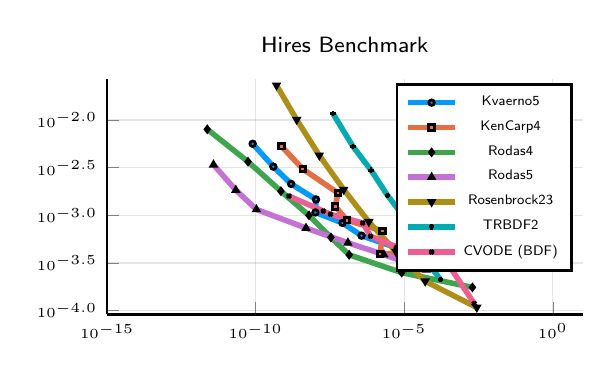
\begin{tikzpicture}[]
\begin{axis}[height = {45.72mm}, title = {Hires Benchmark}, xmin = {1.0e-15}, xmax = {10}, ymax = {0.027253160531968752}, ymode = {log}, unbounded coords=jump,scaled x ticks = false,xlabel style = {font = {\fontsize{5 pt}{6.5 pt}\selectfont}, color = {rgb,1:red,0.00000000;green,0.00000000;blue,0.00000000}, draw opacity = 1.0, rotate = 0.0},log basis x=10,xmajorgrids = true,xtick = {1.0e-15,1.0e-10,1.0e-5,1.0},xticklabels = {$10^{-15}$,$10^{-10}$,$10^{-5}$,$10^{0}$},xtick align = inside,xticklabel style = {font = {\fontsize{5 pt}{6.5 pt}\selectfont}, color = {rgb,1:red,0.00000000;green,0.00000000;blue,0.00000000}, draw opacity = 1.0, rotate = 0.0},x grid style = {color = {rgb,1:red,0.00000000;green,0.00000000;blue,0.00000000},
draw opacity = 0.1,
line width = 0.5,
solid},axis lines* = left,x axis line style = {color = {rgb,1:red,0.00000000;green,0.00000000;blue,0.00000000},
draw opacity = 1.0,
line width = 1,
solid},scaled y ticks = false,ylabel style = {font = {\fontsize{5 pt}{6.5 pt}\selectfont}, color = {rgb,1:red,0.00000000;green,0.00000000;blue,0.00000000}, draw opacity = 1.0, rotate = 0.0},log basis y=10,ymajorgrids = true,ytick = {0.0001,0.00031622776601683794,0.001,0.0031622776601683794,0.01},yticklabels = {$10^{-4.0}$,$10^{-3.5}$,$10^{-3.0}$,$10^{-2.5}$,$10^{-2.0}$},ytick align = inside,yticklabel style = {font = {\fontsize{5 pt}{6.5 pt}\selectfont}, color = {rgb,1:red,0.00000000;green,0.00000000;blue,0.00000000}, draw opacity = 1.0, rotate = 0.0},y grid style = {color = {rgb,1:red,0.00000000;green,0.00000000;blue,0.00000000},
draw opacity = 0.1,
line width = 0.5,
solid},axis lines* = left,y axis line style = {color = {rgb,1:red,0.00000000;green,0.00000000;blue,0.00000000},
draw opacity = 1.0,
line width = 1,
solid},    xshift = 0.0mm,
    yshift = 0.0mm,
    axis background/.style={fill={rgb,1:red,1.00000000;green,1.00000000;blue,1.00000000}}
,title style = {font = {\fontsize{8 pt}{10.4 pt}\selectfont}, color = {rgb,1:red,0.00000000;green,0.00000000;blue,0.00000000}, draw opacity = 1.0, rotate = 0.0},legend style = {color = {rgb,1:red,0.00000000;green,0.00000000;blue,0.00000000},
draw opacity = 1.0,
line width = 1,
solid,fill = {rgb,1:red,1.00000000;green,1.00000000;blue,1.00000000},font = {\fontsize{3 pt}{3.9000000000000004 pt}\selectfont}},colorbar style={title=}, xmode = {log}, ymin = {9.156326857550474e-5}, width = {76.2mm}]\addplot+ [color = {rgb,1:red,0.00000000;green,0.60560316;blue,0.97868012},
draw opacity = 1.0,
line width = 2,
solid,mark = *,
mark size = 1.0,
mark options = {
    color = {rgb,1:red,0.00000000;green,0.00000000;blue,0.00000000}, draw opacity = 1.0,
    fill = {rgb,1:red,0.00000000;green,0.60560316;blue,0.97868012}, fill opacity = 1.0,
    line width = 1,
    rotate = 0,
    solid
}]coordinates {
(6.021709247576974e-6, 0.000451473)
(3.6654161554464015e-7, 0.000610449)
(8.406982627305567e-8, 0.000830366)
(1.0292458800223462e-8, 0.001070496)
(1.0765262187529232e-8, 0.001466483)
(1.571971083372801e-9, 0.002135938)
(3.947373440290987e-10, 0.003241071)
(7.947058958032152e-11, 0.005640182)
};
\addlegendentry{Kvaerno5}
\addplot+ [color = {rgb,1:red,0.88887350;green,0.43564919;blue,0.27812294},
draw opacity = 1.0,
line width = 2,
solid,mark = square*,
mark size = 1.0,
mark options = {
    color = {rgb,1:red,0.00000000;green,0.00000000;blue,0.00000000}, draw opacity = 1.0,
    fill = {rgb,1:red,0.88887350;green,0.43564919;blue,0.27812294}, fill opacity = 1.0,
    line width = 1,
    rotate = 0,
    solid
}]coordinates {
(1.81255015768759e-5, 0.000407062)
(1.5670135007367753e-6, 0.000393158)
(1.840399474366405e-6, 0.000685586)
(1.1944650623573266e-7, 0.00088648)
(4.747191733012903e-8, 0.001239116)
(5.9245300969584005e-8, 0.001711633)
(3.856480277308183e-9, 0.003065304)
(7.409066819333049e-10, 0.005313971)
};
\addlegendentry{KenCarp4}
\addplot+ [color = {rgb,1:red,0.24222430;green,0.64327509;blue,0.30444865},
draw opacity = 1.0,
line width = 2,
solid,mark = diamond*,
mark size = 1.0,
mark options = {
    color = {rgb,1:red,0.00000000;green,0.00000000;blue,0.00000000}, draw opacity = 1.0,
    fill = {rgb,1:red,0.24222430;green,0.64327509;blue,0.30444865}, fill opacity = 1.0,
    line width = 1,
    rotate = 0,
    solid
}]coordinates {
(0.001976703313890534, 0.000174804)
(8.261808154441106e-6, 0.000249679)
(1.4030378597148392e-7, 0.000384394)
(3.417897963119001e-8, 0.000585014)
(6.208014488397182e-9, 0.000998205)
(7.092762382161896e-10, 0.001792547)
(5.552737426356121e-11, 0.0036571)
(2.3526602808786453e-12, 0.008011298)
};
\addlegendentry{Rodas4}
\addplot+ [color = {rgb,1:red,0.76444018;green,0.44411178;blue,0.82429754},
draw opacity = 1.0,
line width = 2,
solid,mark = triangle*,
mark size = 1.0,
mark options = {
    color = {rgb,1:red,0.00000000;green,0.00000000;blue,0.00000000}, draw opacity = 1.0,
    fill = {rgb,1:red,0.76444018;green,0.44411178;blue,0.82429754}, fill opacity = 1.0,
    line width = 1,
    rotate = 0,
    solid
}]coordinates {
(5.5313349654323375e-5, 0.000267801)
(2.0698583045638375e-6, 0.000385908)
(1.273777832893035e-7, 0.000514331)
(4.963568137598741e-9, 0.00073445)
(1.0620345121101947e-10, 0.001151617)
(2.155587069518211e-11, 0.001841238)
(3.81783070699845e-12, 0.003396517)
};
\addlegendentry{Rodas5}
\addplot+ [color = {rgb,1:red,0.67554396;green,0.55566233;blue,0.09423434},
draw opacity = 1.0,
line width = 2,
solid,mark = triangle*,
mark size = 1.0,
mark options = {
    color = {rgb,1:red,0.00000000;green,0.00000000;blue,0.00000000}, draw opacity = 1.0,
    fill = {rgb,1:red,0.67554396;green,0.55566233;blue,0.09423434}, fill opacity = 1.0,
    line width = 1,
    rotate = 180,
    solid
}]coordinates {
(0.002767244573521482, 0.00010758)
(5.09096502734123e-5, 0.00020294)
(5.264958855745958e-6, 0.000414579)
(6.454495975662898e-7, 0.000855006)
(9.200049242726101e-8, 0.001861111)
(1.3868650354178758e-8, 0.004261763)
(2.4142651465262636e-9, 0.010094259)
(5.051997646455969e-10, 0.023195654)
};
\addlegendentry{Rosenbrock23}
\addplot+ [color = {rgb,1:red,0.00000048;green,0.66575898;blue,0.68099695},
draw opacity = 1.0,
line width = 2,
solid,mark = +,
mark size = 1.0,
mark options = {
    color = {rgb,1:red,0.00000000;green,0.00000000;blue,0.00000000}, draw opacity = 1.0,
    fill = {rgb,1:red,0.00000048;green,0.66575898;blue,0.68099695}, fill opacity = 1.0,
    line width = 1,
    rotate = 0,
    solid
}]coordinates {
(0.00016645669386475468, 0.000210435)
(7.931074455456665e-5, 0.000287057)
(2.6863558101760393e-5, 0.000504215)
(1.4740960149198529e-5, 0.000815383)
(2.7389708872361167e-6, 0.001619555)
(7.64907558421203e-7, 0.00297628)
(1.8729010502077252e-7, 0.005294634)
(4.030901710171368e-8, 0.011667364)
};
\addlegendentry{TRBDF2}
\addplot+ [color = {rgb,1:red,0.93076749;green,0.36747719;blue,0.57576997},
draw opacity = 1.0,
line width = 2,
solid,mark = x,
mark size = 1.0,
mark options = {
    color = {rgb,1:red,0.00000000;green,0.00000000;blue,0.00000000}, draw opacity = 1.0,
    fill = {rgb,1:red,0.93076749;green,0.36747719;blue,0.57576997}, fill opacity = 1.0,
    line width = 1,
    rotate = 0,
    solid
}]coordinates {
(0.002255854552039932, 0.000118357)
(0.0003103462027842327, 0.000301927)
(5.115149147238372e-5, 0.000352446)
(7.368792629530713e-7, 0.000602032)
(4.018912866480474e-7, 0.000829604)
(3.2932465473851896e-8, 0.001025623)
(1.8806520926542736e-8, 0.001107969)
(1.323761427214195e-9, 0.001592726)
};
\addlegendentry{CVODE (BDF)}
\end{axis}

\end{tikzpicture}

  \end{center}
}

\boxit{below of = box3, col=1, name=box4}{Implicit-Explicit (Multirate) and
  Exponential Methods}{
  Implicit-explicit methods solve the equations in the form of
  \[
    u' = f_1(u,t) + f_2(u, t),
  \]
  where $f_1$ is stiff, and $f_2$ is non-stiff.
  If the $f_1$ function is
  non-linear, one can use an additive Runge-Kutta method. If the $f_1$ function
  is linear, then one solve the linear part exactly by using an exponential
  Runge-Kutta method.
  %Exponential Runge-Kutta integrators use linear
  %combinations of matrix $\phi$ function, where $\phi$ functions are defined by
  %\[
  %  \phi_0(A) = e^A, \quad \phi_l(A) = \frac{1}{(l-1)!}\int_0^1
  %  e^{(1-\theta)A}\theta^{l-1}\; d\theta, \quad l = 1,2,\cdots.
  %\]
  %One popular method of computing the matrix $\phi$ function is to use adaptive
  %Krylov subspace methods, which is to find $\phi(z)v$ in the space
  %\[
  %  \text{span}\{z, Az, A^2z, \cdots, A^{m-1}z\},
  %\]
  %where $m$ adapts to balance the computational effort and accuracy.
  \begin{center}
    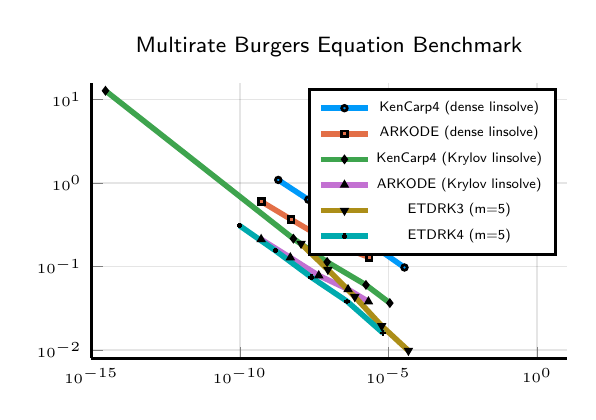
\begin{tikzpicture}[]
\begin{axis}[height = {50.8mm}, title = {Multirate Burgers Equation Benchmark}, xmin = {1.0e-15}, xmax = {10}, ymax = {15.776844127916583}, ymode = {log}, unbounded coords=jump,scaled x ticks = false,xlabel style = {font = {\fontsize{5 pt}{6.5 pt}\selectfont}, color = {rgb,1:red,0.00000000;green,0.00000000;blue,0.00000000}, draw opacity = 1.0, rotate = 0.0},log basis x=10,xmajorgrids = true,xtick = {1.0e-15,1.0e-10,1.0e-5,1.0},xticklabels = {$10^{-15}$,$10^{-10}$,$10^{-5}$,$10^{0}$},xtick align = inside,xticklabel style = {font = {\fontsize{5 pt}{6.5 pt}\selectfont}, color = {rgb,1:red,0.00000000;green,0.00000000;blue,0.00000000}, draw opacity = 1.0, rotate = 0.0},x grid style = {color = {rgb,1:red,0.00000000;green,0.00000000;blue,0.00000000},
draw opacity = 0.1,
line width = 0.5,
solid},axis lines* = left,x axis line style = {color = {rgb,1:red,0.00000000;green,0.00000000;blue,0.00000000},
draw opacity = 1.0,
line width = 1,
solid},scaled y ticks = false,ylabel style = {font = {\fontsize{5 pt}{6.5 pt}\selectfont}, color = {rgb,1:red,0.00000000;green,0.00000000;blue,0.00000000}, draw opacity = 1.0, rotate = 0.0},log basis y=10,ymajorgrids = true,ytick = {0.01,0.1,1.0,10.0},yticklabels = {$10^{-2}$,$10^{-1}$,$10^{0}$,$10^{1}$},ytick align = inside,yticklabel style = {font = {\fontsize{5 pt}{6.5 pt}\selectfont}, color = {rgb,1:red,0.00000000;green,0.00000000;blue,0.00000000}, draw opacity = 1.0, rotate = 0.0},y grid style = {color = {rgb,1:red,0.00000000;green,0.00000000;blue,0.00000000},
draw opacity = 0.1,
line width = 0.5,
solid},axis lines* = left,y axis line style = {color = {rgb,1:red,0.00000000;green,0.00000000;blue,0.00000000},
draw opacity = 1.0,
line width = 1,
solid},    xshift = 0.0mm,
    yshift = 0.0mm,
    axis background/.style={fill={rgb,1:red,1.00000000;green,1.00000000;blue,1.00000000}}
,title style = {font = {\fontsize{8 pt}{10.4 pt}\selectfont}, color = {rgb,1:red,0.00000000;green,0.00000000;blue,0.00000000}, draw opacity = 1.0, rotate = 0.0},legend style = {color = {rgb,1:red,0.00000000;green,0.00000000;blue,0.00000000},
draw opacity = 1.0,
line width = 1,
solid,fill = {rgb,1:red,1.00000000;green,1.00000000;blue,1.00000000},font = {\fontsize{3 pt}{3.9000000000000004 pt}\selectfont}},colorbar style={title=}, xmode = {log}, ymin = {0.007904077109128715}, width = {76.2mm}]\addplot+ [color = {rgb,1:red,0.00000000;green,0.60560316;blue,0.97868012},
draw opacity = 1.0,
line width = 2,
solid,mark = *,
mark size = 1.0,
mark options = {
    color = {rgb,1:red,0.00000000;green,0.00000000;blue,0.00000000}, draw opacity = 1.0,
    fill = {rgb,1:red,0.00000000;green,0.60560316;blue,0.97868012}, fill opacity = 1.0,
    line width = 1,
    rotate = 0,
    solid
}]coordinates {
(3.4648103383872526e-5, 0.097071093)
(2.7814951199546194e-6, 0.181906111)
(2.118105787153261e-7, 0.341356229)
(2.0098094007543837e-8, 0.631136249)
(1.959516371706548e-9, 1.086916523)
};
\addlegendentry{KenCarp4 (dense linsolve)}
\addplot+ [color = {rgb,1:red,0.88887350;green,0.43564919;blue,0.27812294},
draw opacity = 1.0,
line width = 2,
solid,mark = square*,
mark size = 1.0,
mark options = {
    color = {rgb,1:red,0.00000000;green,0.00000000;blue,0.00000000}, draw opacity = 1.0,
    fill = {rgb,1:red,0.88887350;green,0.43564919;blue,0.27812294}, fill opacity = 1.0,
    line width = 1,
    rotate = 0,
    solid
}]coordinates {
(2.2707765343744006e-6, 0.128150168)
(3.6788876697267834e-7, 0.164177227)
(4.455204624858925e-8, 0.234420187)
(5.352076989144092e-9, 0.364909279)
(5.35662117817959e-10, 0.597057398)
};
\addlegendentry{ARKODE (dense linsolve)}
\addplot+ [color = {rgb,1:red,0.24222430;green,0.64327509;blue,0.30444865},
draw opacity = 1.0,
line width = 2,
solid,mark = diamond*,
mark size = 1.0,
mark options = {
    color = {rgb,1:red,0.00000000;green,0.00000000;blue,0.00000000}, draw opacity = 1.0,
    fill = {rgb,1:red,0.24222430;green,0.64327509;blue,0.30444865}, fill opacity = 1.0,
    line width = 1,
    rotate = 0,
    solid
}]coordinates {
(1.113318376312209e-5, 0.036404373)
(1.7477558362010042e-6, 0.060001805)
(8.624006797682366e-8, 0.113135202)
(6.321267939163031e-9, 0.215084504)
(2.9957635733888373e-15, 12.72386716)
};
\addlegendentry{KenCarp4 (Krylov linsolve)}
\addplot+ [color = {rgb,1:red,0.76444018;green,0.44411178;blue,0.82429754},
draw opacity = 1.0,
line width = 2,
solid,mark = triangle*,
mark size = 1.0,
mark options = {
    color = {rgb,1:red,0.00000000;green,0.00000000;blue,0.00000000}, draw opacity = 1.0,
    fill = {rgb,1:red,0.76444018;green,0.44411178;blue,0.82429754}, fill opacity = 1.0,
    line width = 1,
    rotate = 0,
    solid
}]coordinates {
(2.118411571520636e-6, 0.037960327)
(4.373166746363195e-7, 0.053110761)
(4.5087873239683744e-8, 0.077791497)
(4.9772815346311464e-9, 0.127812883)
(5.193626980967097e-10, 0.2114173)
};
\addlegendentry{ARKODE (Krylov linsolve)}
\addplot+ [color = {rgb,1:red,0.67554396;green,0.55566233;blue,0.09423434},
draw opacity = 1.0,
line width = 2,
solid,mark = triangle*,
mark size = 1.0,
mark options = {
    color = {rgb,1:red,0.00000000;green,0.00000000;blue,0.00000000}, draw opacity = 1.0,
    fill = {rgb,1:red,0.67554396;green,0.55566233;blue,0.09423434}, fill opacity = 1.0,
    line width = 1,
    rotate = 180,
    solid
}]coordinates {
(4.693599813090348e-5, 0.009800589)
(5.914208264839906e-6, 0.019406029)
(7.360331501650721e-7, 0.043309185)
(9.167567766999955e-8, 0.091419605)
(1.1435992218461219e-8, 0.187469357)
};
\addlegendentry{ETDRK3 (m=5)}
\addplot+ [color = {rgb,1:red,0.00000048;green,0.66575898;blue,0.68099695},
draw opacity = 1.0,
line width = 2,
solid,mark = +,
mark size = 1.0,
mark options = {
    color = {rgb,1:red,0.00000000;green,0.00000000;blue,0.00000000}, draw opacity = 1.0,
    fill = {rgb,1:red,0.00000048;green,0.66575898;blue,0.68099695}, fill opacity = 1.0,
    line width = 1,
    rotate = 0,
    solid
}]coordinates {
(6.535650828647287e-6, 0.015969848)
(4.054496929215464e-7, 0.038185714)
(2.5120547006198278e-8, 0.074337009)
(1.5617106897893295e-9, 0.154802398)
(9.732799825817218e-11, 0.308371751)
};
\addlegendentry{ETDRK4 (m=5)}
\end{axis}

\end{tikzpicture}

  \end{center}
}

%\boxit{below of = box4, col = 1, name=solution}{Exponential Propagation Iterative
%  Runge-Kutta (EPIRK) Methods}{
%}

\boxit{at top,col = 2, name=events}{Disadvantages of BDF Method}{
  BDF method has a very high starting cost, which makes it not suitable for QsP
  modeling. Here is a plot to show that BDF method is inefficient with the
  presence of events.
  \begin{center}
    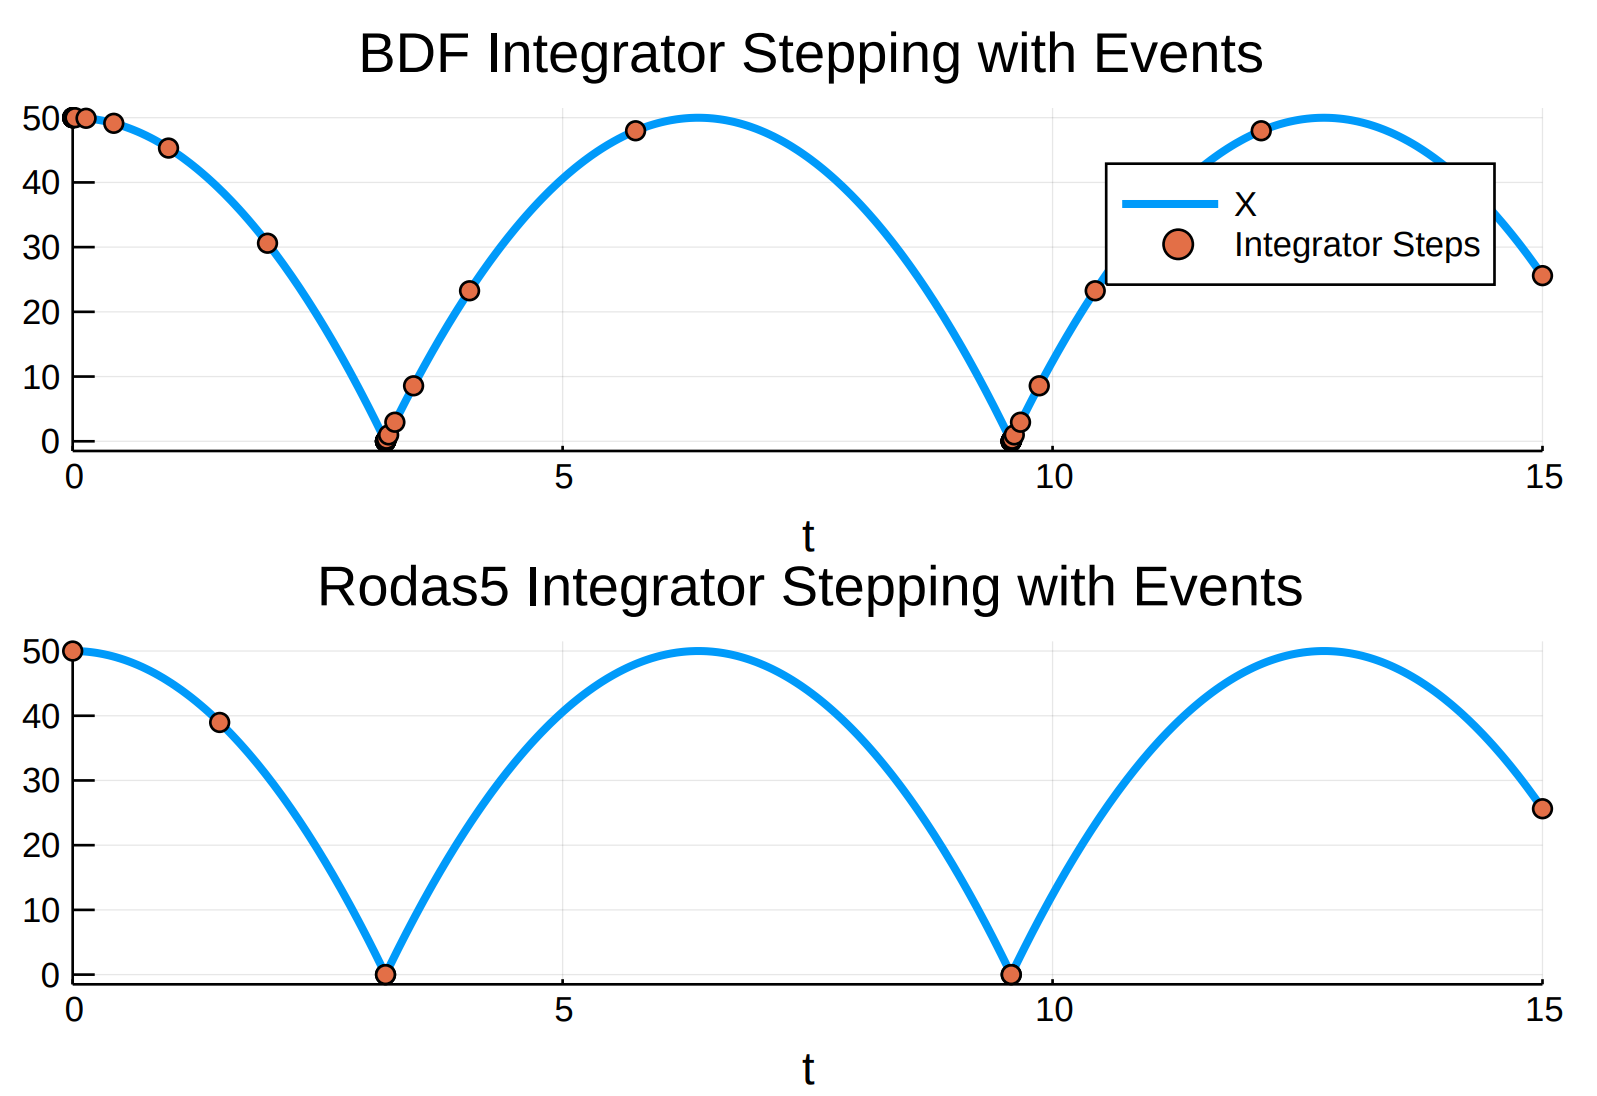
\includegraphics[width=200px,height=150px]{2019-04-22-164648_1597x1096_escrotum.png}
  \end{center}
  \vspace{3pt}

  We can see that because BDF method needs history states, it has to restart
  from the first order every time when there is an event. Therefore, it has to
  take every small time steps to avoid step rejections.

  \vspace{5pt}
  High order BDF method is not A-stable, thus using high order BDFs could lead
  to oscillatory solution because of the lack of A-stability.
  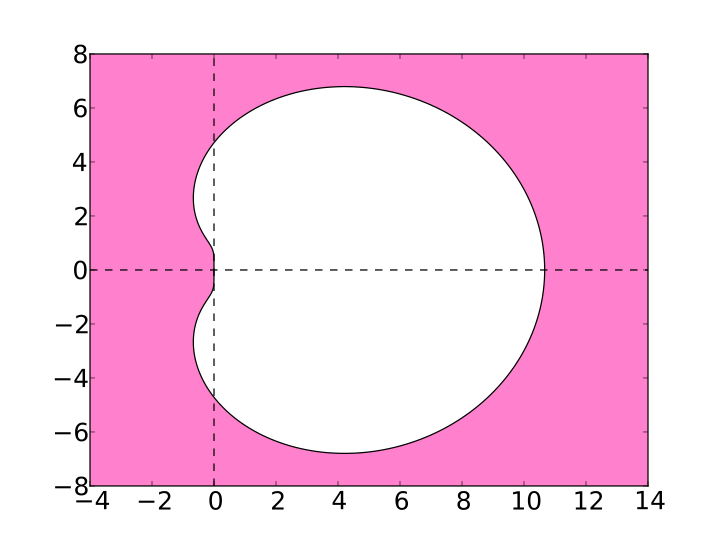
\includegraphics[width=50px,height=50px]{Stability_region_for_BDF4.png}
}

\boxit{below of = events,col = 2, name=conc}{Conclusion}{
  \begin{itemize}
    \item We have sped up one of Pfizer's cardiac QsP models by 26 times by
      translating Matlab to Julia and use a fifth order Rosenbrock method.
    \item Rosenbrock methods tend to perform better than BDF for small models.
    \item With the presence of frequent events, one should consider implicit RK
      or Rosenbrock to avoid inefficiency.
    \item Exponential integrators are very worth looking into.
    \item Jacobian reuse is crucial for performance.
  \end{itemize}
  \vspace{10pt}
}

\boxit{below of = conc,col = 2, name=ack}{Acknowledgments}{
  We would like to acknowledge Julia Computing and the University of Maryland
  Baltimore's Center for Translational Medicine for sponsoring the development
  of OrdinaryDiffEq and PuMaS.
  \vspace{9.5pt}
}

\end{document}
